

\providecommand{\graphscale}{0.6}


\newcommand{\dirfunc}[3]{ \frac{ \prod_{#1}^{#2} \g{ #3 } } { \g{ \sum_{#1}^{#2} #3 }}}
\newcommand{\dirnum}[4]{ \frac{\g{ #3 }}{#4} \prod_{#1}^{#2} }
\newcommand{\dirden}[3]{ \g{ \sum_{#1}^{#2} #3 } }


\begin{frame}

	\frametitle{Why topic models?}

	\begin{columns}

	\column{.3\linewidth}

	
\includegraphics[width=1\linewidth]{topic_models/newspapers}

	\column{.55\linewidth}

	\begin{itemize}
		\item Suppose you have a huge number of documents
		\item Want to know what's going on
		\item Can't read them all (e.g. every New York Times article from the 90's)
		\item Topic models offer a way to get a corpus-level view of major themes
		\pause
		\item Unsupervised
	\end{itemize}


	\end{columns}

\end{frame}

\frame{
\begin{center}
\frametitle{Conceptual Approach}
From an \textbf<1>{input corpus} and number of topics \textbf<1>{$K$} $\rightarrow$ \textbf<2>{words to topics} \\
\only<1>{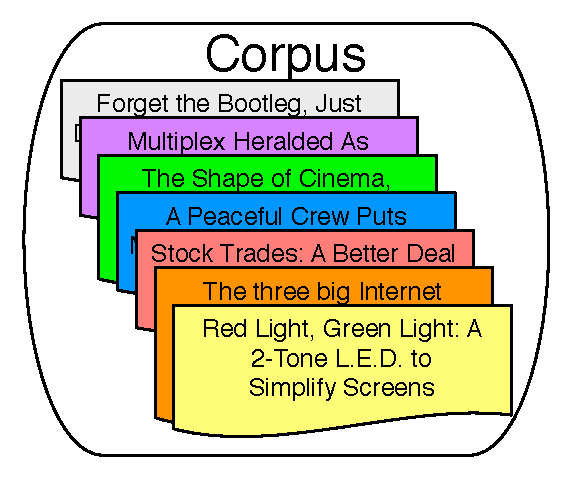
\includegraphics[width=0.6\linewidth]{reading_tea_leaves/figures/heldout_0} }
\only<2>{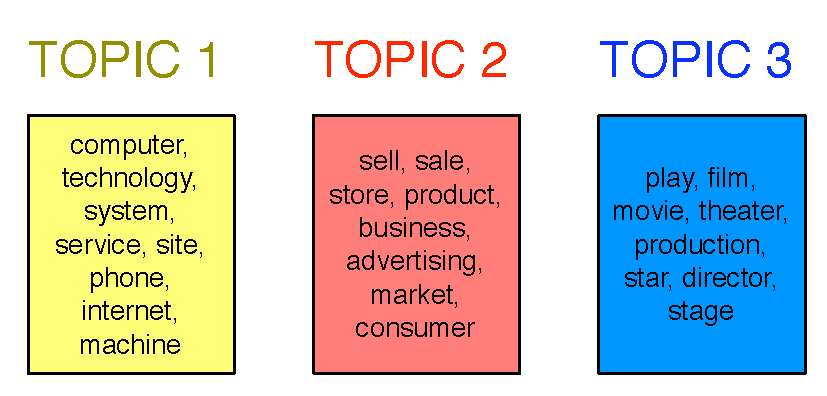
\includegraphics[width=0.9\linewidth]{reading_tea_leaves/figures/nyt_topics_wide}}
\end{center}
}

\frame{\frametitle{Conceptual Approach}

\begin{itemize}
\item For each document, what topics are expressed by that document?

\begin{center}
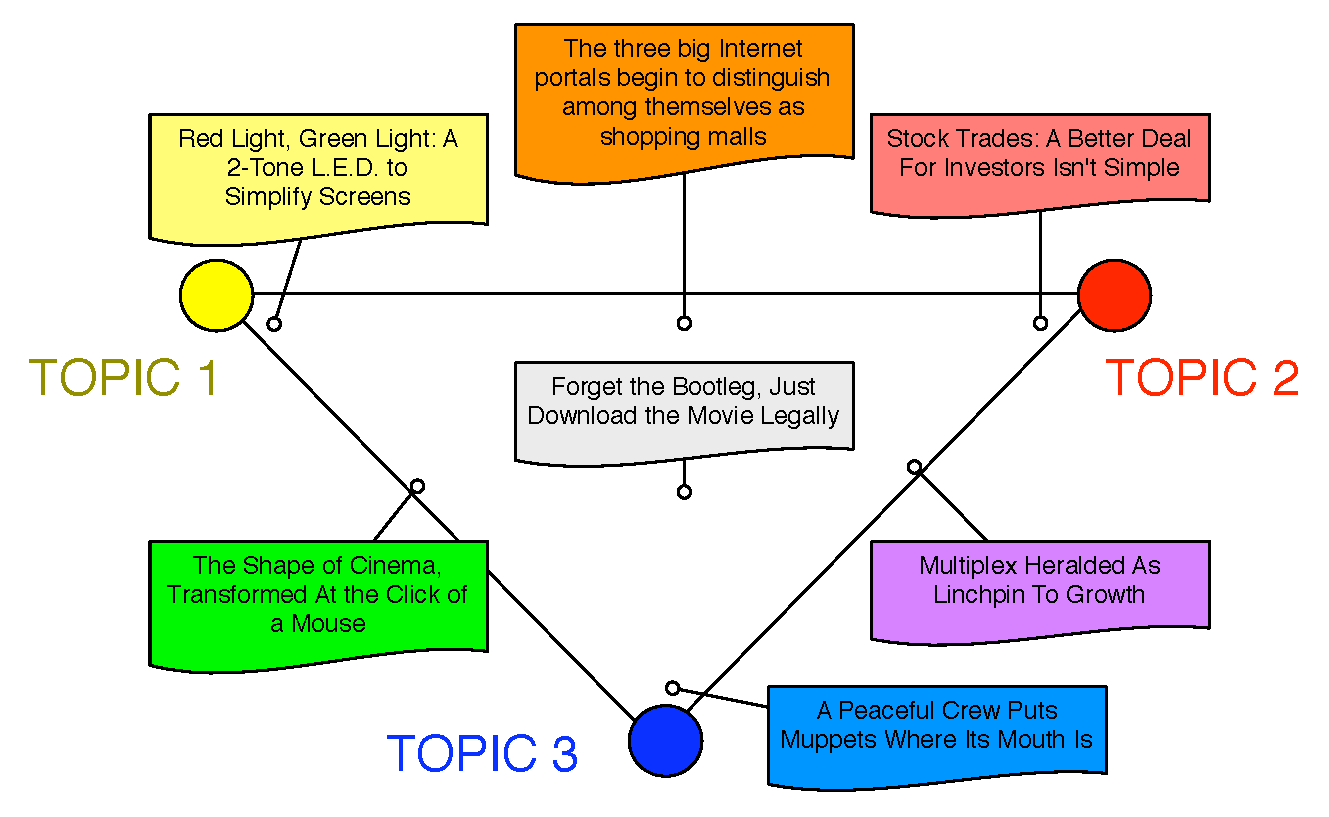
\includegraphics[width=0.9\linewidth]{topic_models/nyt_documents}
\end{center}

\end{itemize}
}

\iflong

\begin{frame}

\frametitle{Topics from \emph{Science}}

\begin{center}
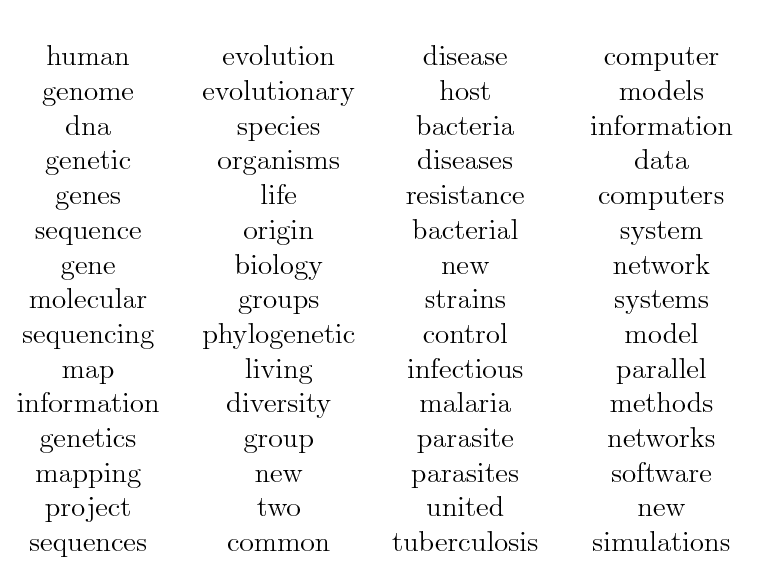
\includegraphics[width=0.8\linewidth]{topic_models/example_topics}
\end{center}

\end{frame}


\begin{frame}

\frametitle{Why should you care?}

\begin{itemize}
\item Neat way to explore / understand corpus collections
\begin{itemize}
	\item E-discovery
	\item Social media
	\item Scientific data
\end{itemize}
\item NLP Applications
\begin{itemize}
   \item POS Tagging~\cite{toutanova-08}
   \item Word Sense Disambiguation~\cite{boyd-graber-07}
   \item Word Sense Induction~\cite{brody-09}
   \item Discourse Segmentation~\cite{purver-06}
\end{itemize}
\item Psychology~\cite{griffiths-07}: word meaning, polysemy
\item Inference is (relatively) simple
\end{itemize}

\end{frame}

\frame
{
  \frametitle{Matrix Factorization Approach}

\begin{center}
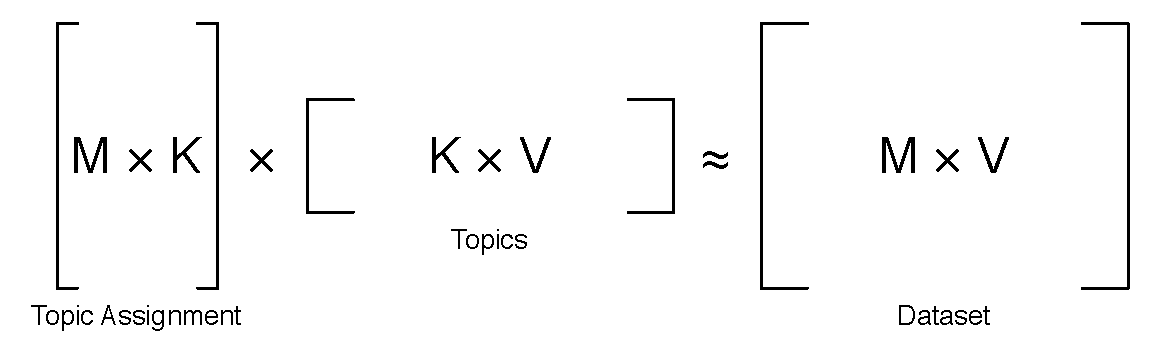
\includegraphics[width=0.9\linewidth]{topic_models/factorization.pdf}
\end{center}

\begin{columns}
\column{.5\textwidth}
\begin{block}{}
	\begin{itemize}
		\item[K] Number of topics
		\item[M] Number of documents
		\item[V] Size of vocabulary
	\end{itemize}
\end{block}
\column{.5\textwidth}
\pause
\begin{itemize}
\item If you use singular value decomposition (SVD), this technique is called latent semantic analysis.
\item Popular in information retrieval.
\end{itemize}
\end{columns}

}

\begin{frame}

\frametitle{Alternative: Generative Model}

\begin{itemize}
  \item How your data came to be
  \item Sequence of Probabilistic Steps
  \item Posterior Inference
    \pause
  \item Blei, Ng, Jordan.  Latent {\bf Dirichlet} Allocation.  JMLR, 2003.
\end{itemize}

\end{frame}

\begin{frame}
	\frametitle{Multinomial Distribution}

	\begin{itemize}
		\item Distribution over discrete outcomes
		\item Represented by non-negative vector that sums to one
		\item Picture representation
	\begin{center}
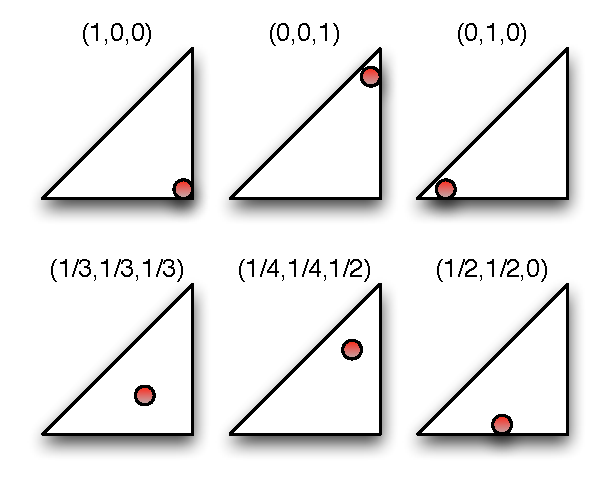
\includegraphics[width=0.4\linewidth]{topic_models/multinomial}
	\end{center}
		\pause
		\item Come from a Dirichlet distribution

	\end{itemize}


\end{frame}

\begin{frame}

\frametitle{Dirichlet Distribution}

\begin{center}
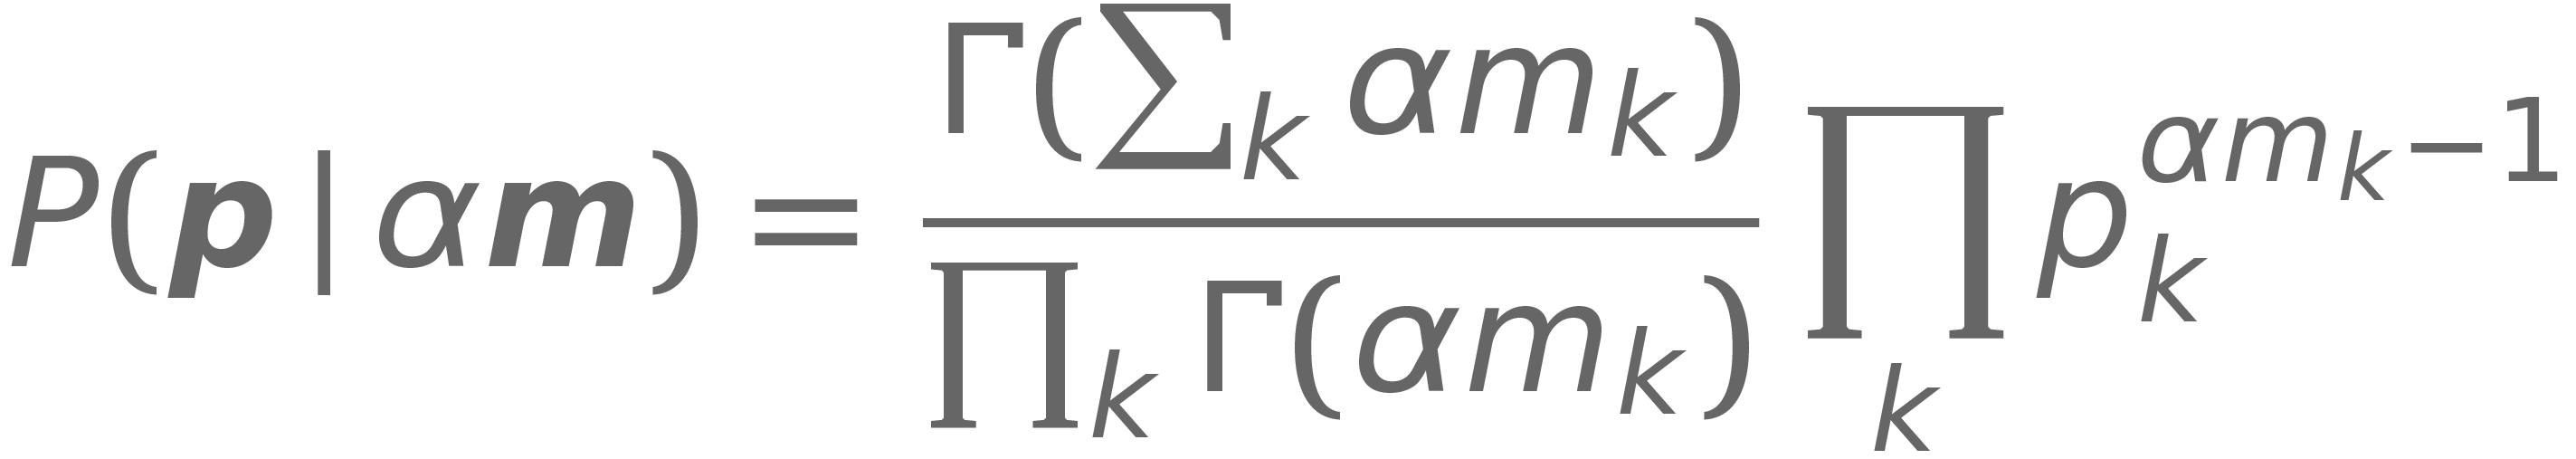
\includegraphics[width=0.4\linewidth]{topic_models/equations/dirichlet} \\ \bigskip
\pause
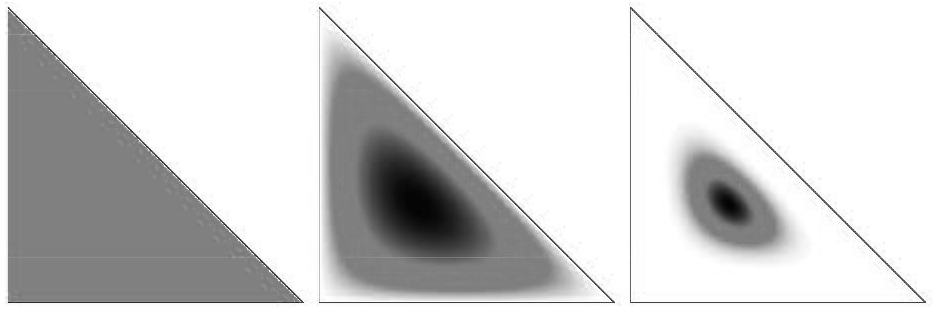
\includegraphics[width=0.6\linewidth]{topic_models/dirichlet_1} \\
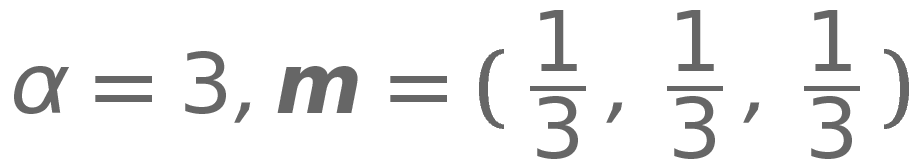
\includegraphics[width=0.2\linewidth]{topic_models/equations/dirichlet_params_1} 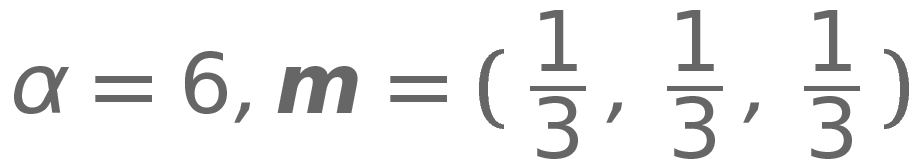
\includegraphics[width=0.2\linewidth]{topic_models/equations/dirichlet_params_2} 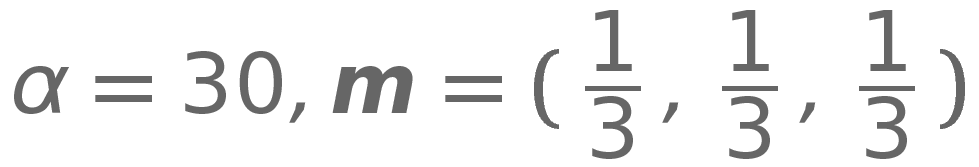
\includegraphics[width=0.2\linewidth]{topic_models/equations/dirichlet_params_3} \\
\pause
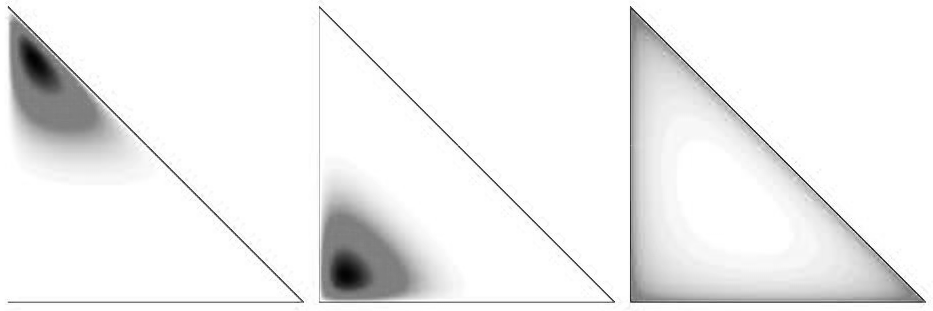
\includegraphics[width=0.6\linewidth]{topic_models/dirichlet_2} \\
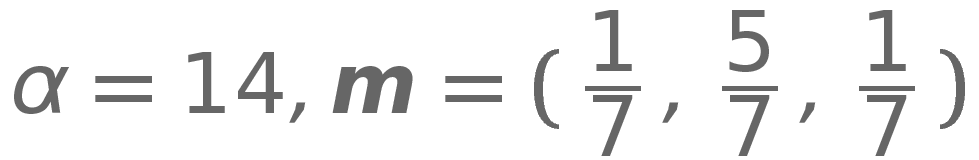
\includegraphics[width=0.2\linewidth]{topic_models/equations/dirichlet_params_4} 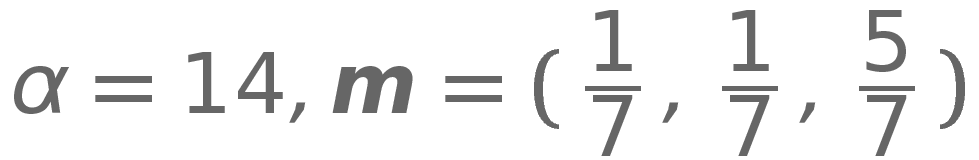
\includegraphics[width=0.2\linewidth]{topic_models/equations/dirichlet_params_5} 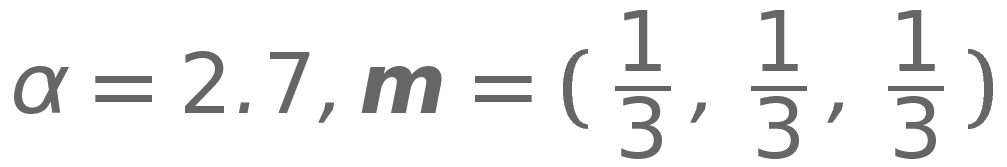
\includegraphics[width=0.2\linewidth]{topic_models/equations/dirichlet_params_6} \\
\end{center}

\end{frame}

\begin{frame}
\frametitle{Dirichlet Distribution}
\begin{center}
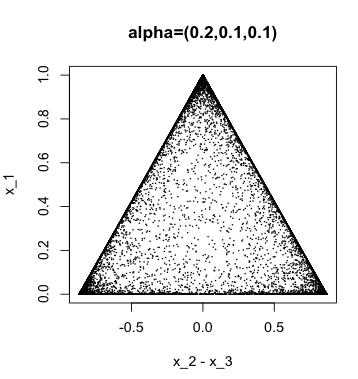
\includegraphics[width=0.5\linewidth]{topic_models/sparsity}
\end{center}
\end{frame}

\fi
\ifconjugacy

\begin{frame}
\frametitle{Dirichlet Distribution}
\begin{itemize}
  \item If ${\bm \phi} \sim \Dir(\alpha)$, ${\bm w} \sim \Mult(\phi)$, and $n_k = |\{ w_i : w_i = k\}|$ then
  \begin{align}
  	p(\phi | \alpha, {\bm w}) & \propto p({\bm w} | \phi) p(\phi | \alpha) \\
	                       & \propto  \prod_{k} \phi^{n_k} \pause  \prod_k { \phi^{\alpha_k - 1}} \\
	                       & \propto \prod_k \phi^{\alpha_k + n_k - 1}
  \end{align}
  \item Conjugacy: this {\bf posterior} has the same form as the {\bf prior}
\end{itemize}
\end{frame}

\fi

\ifhighlevel

\else

\begin{frame}{Generative Model}
	\only<1> {   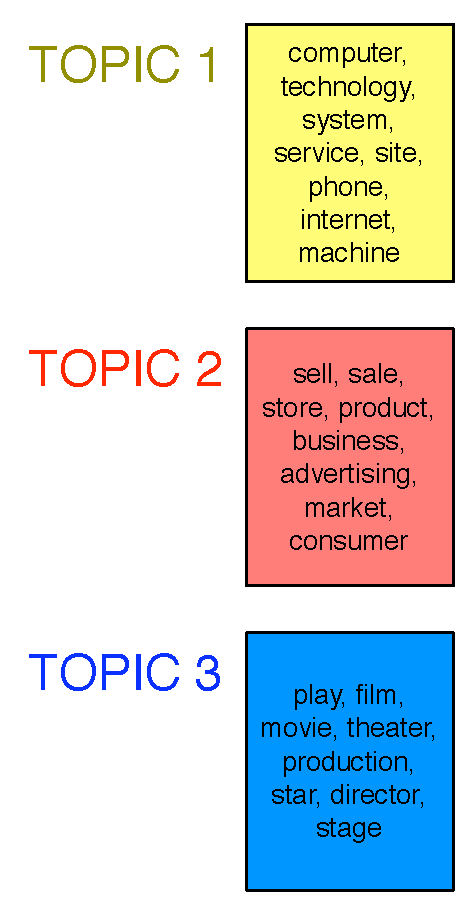
\includegraphics[width=.8\linewidth]{topic_models/nyt_topics}  }
	\only<2> {   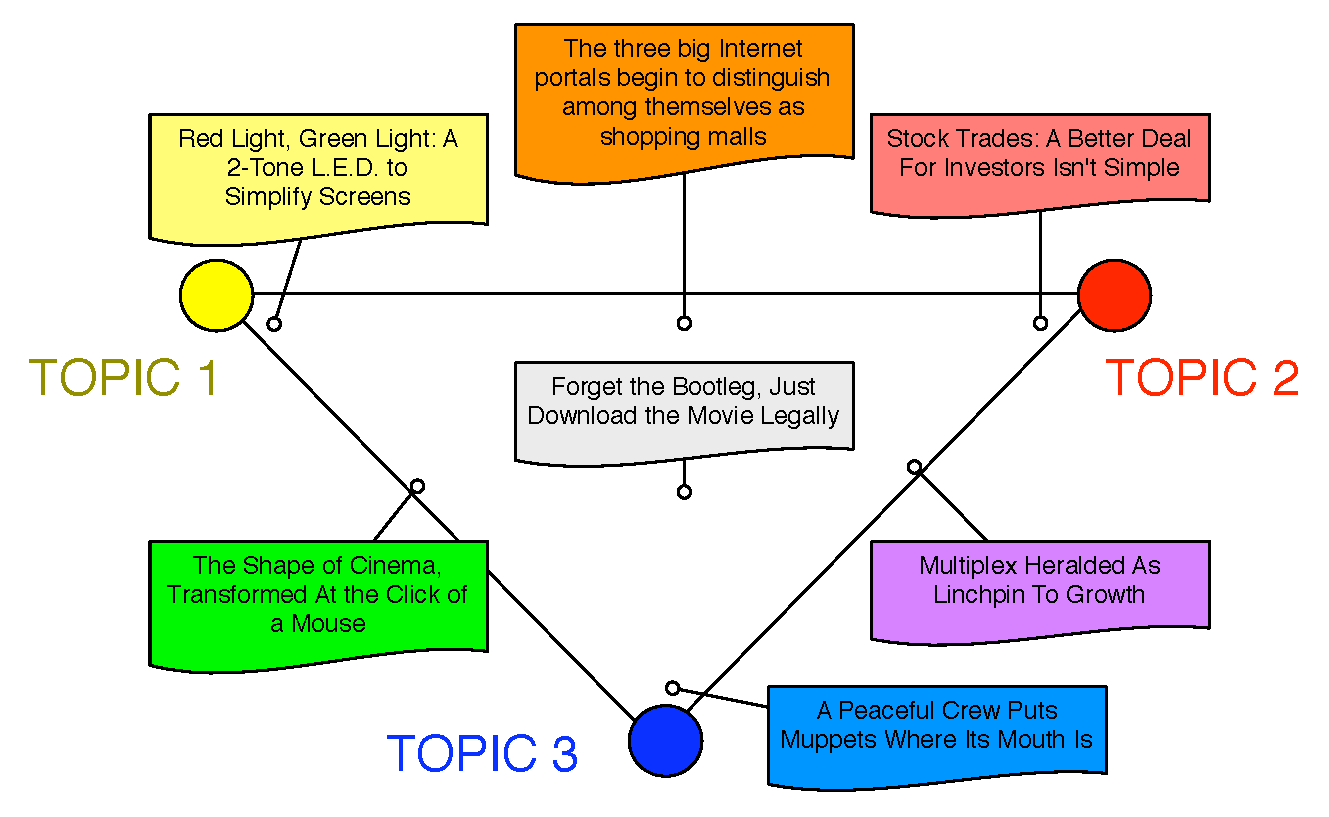
\includegraphics[width=.8\linewidth]{topic_models/nyt_documents}  }
	\only<3> {   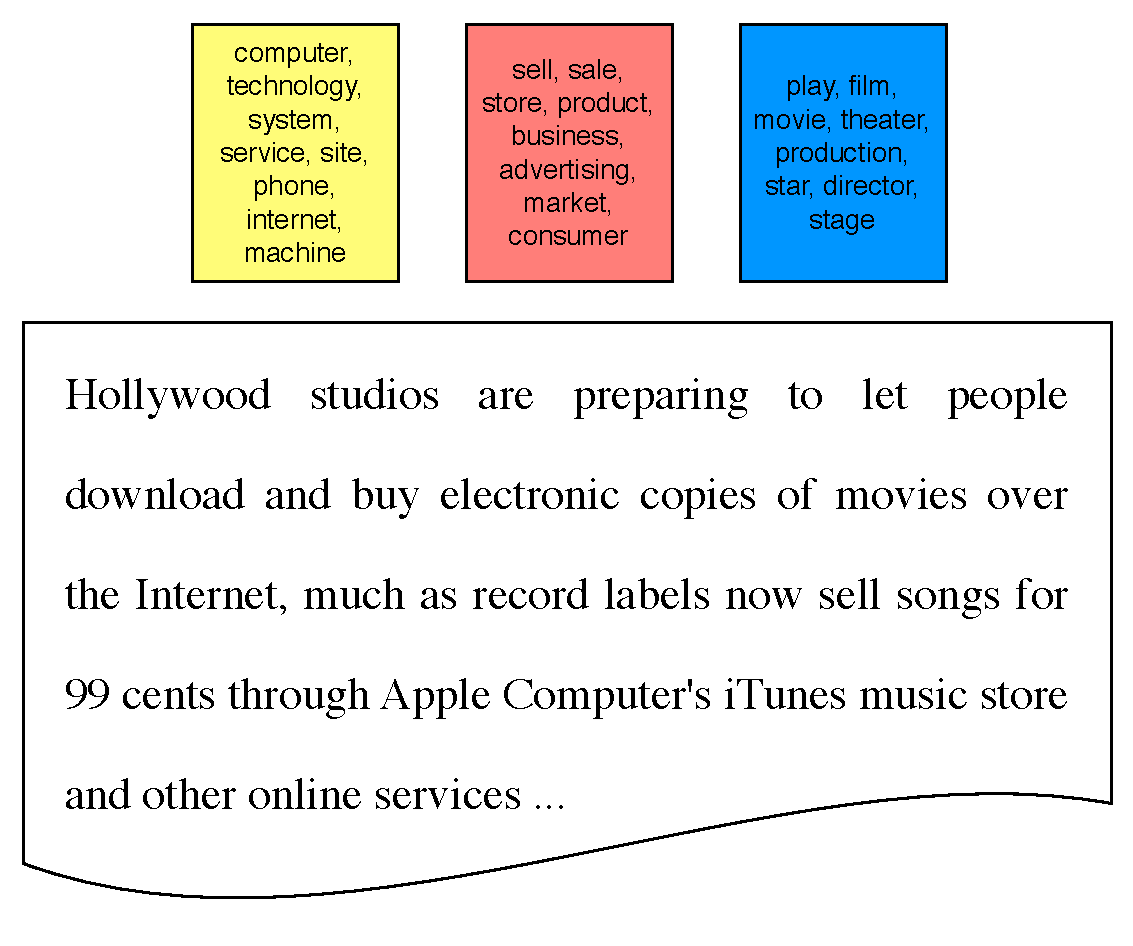
\includegraphics[width=.8\linewidth]{topic_models/inference_0}  }
	\only<4> {   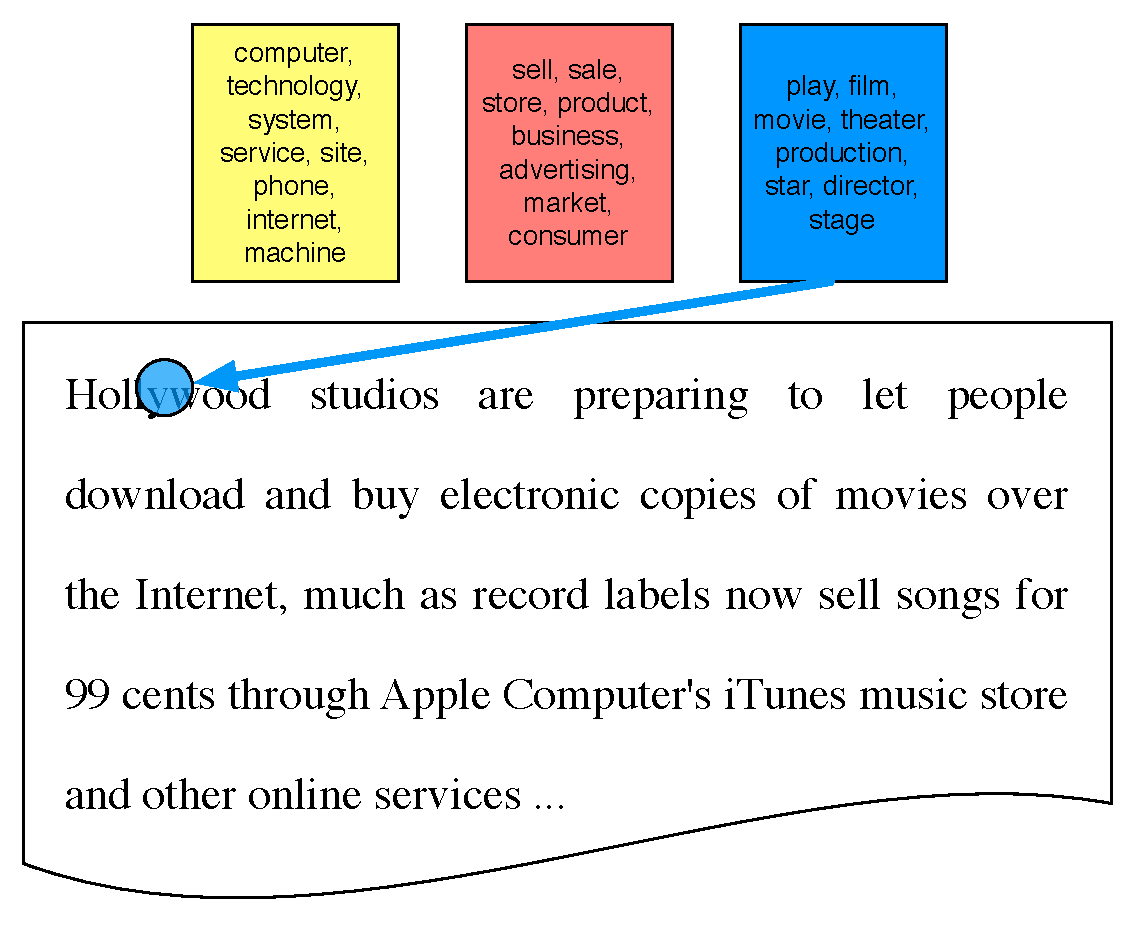
\includegraphics[width=.8\linewidth]{topic_models/inference_1}  }
	\only<5> {   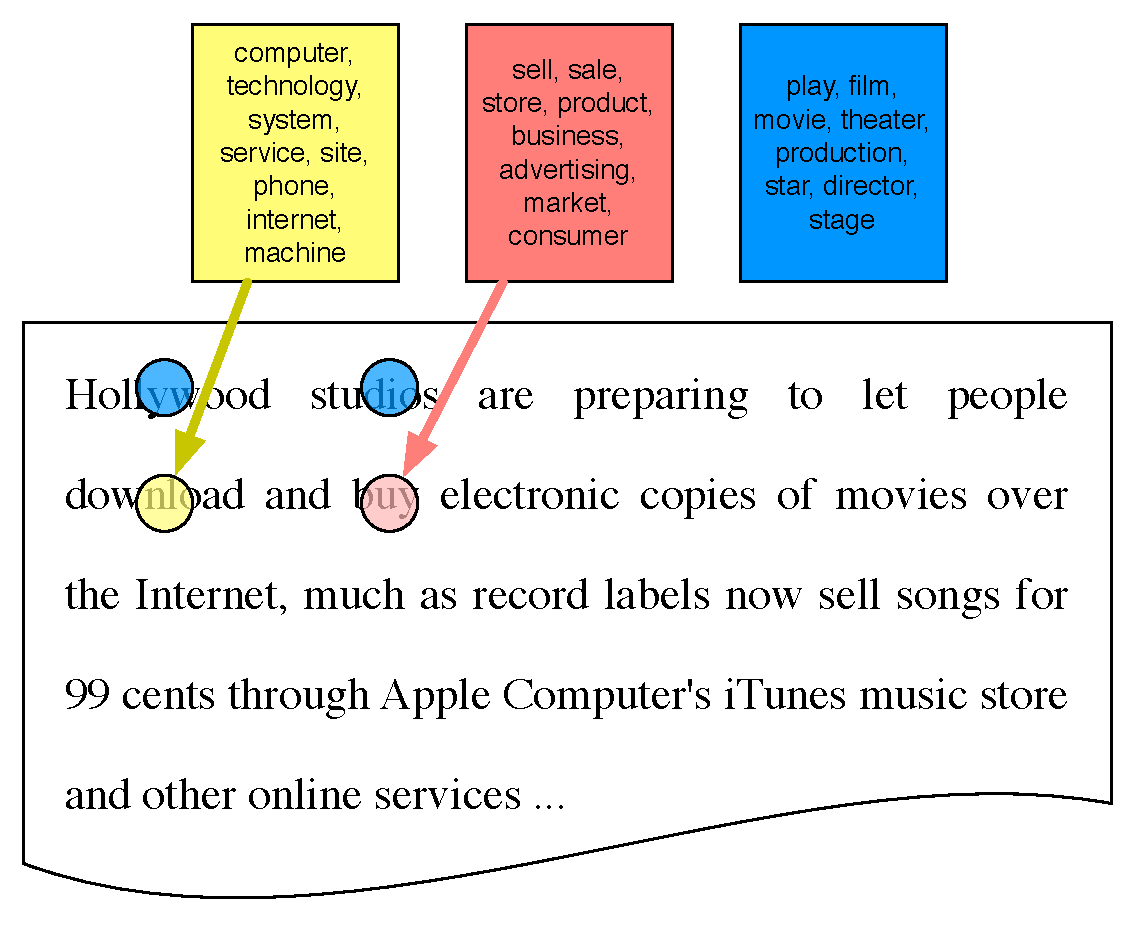
\includegraphics[width=.8\linewidth]{topic_models/inference_2}  }
	\only<6> {   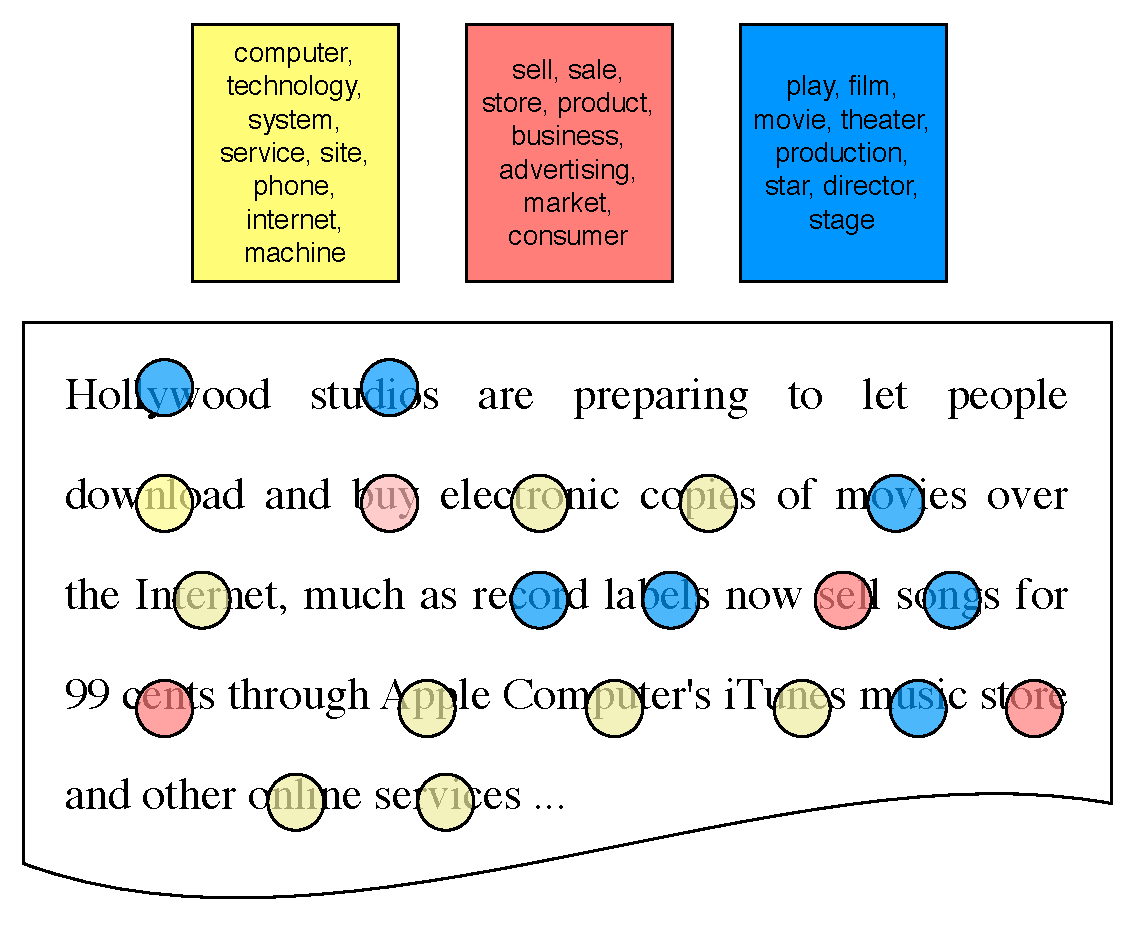
\includegraphics[width=.8\linewidth]{topic_models/inference_3}  }
	\only<7> {   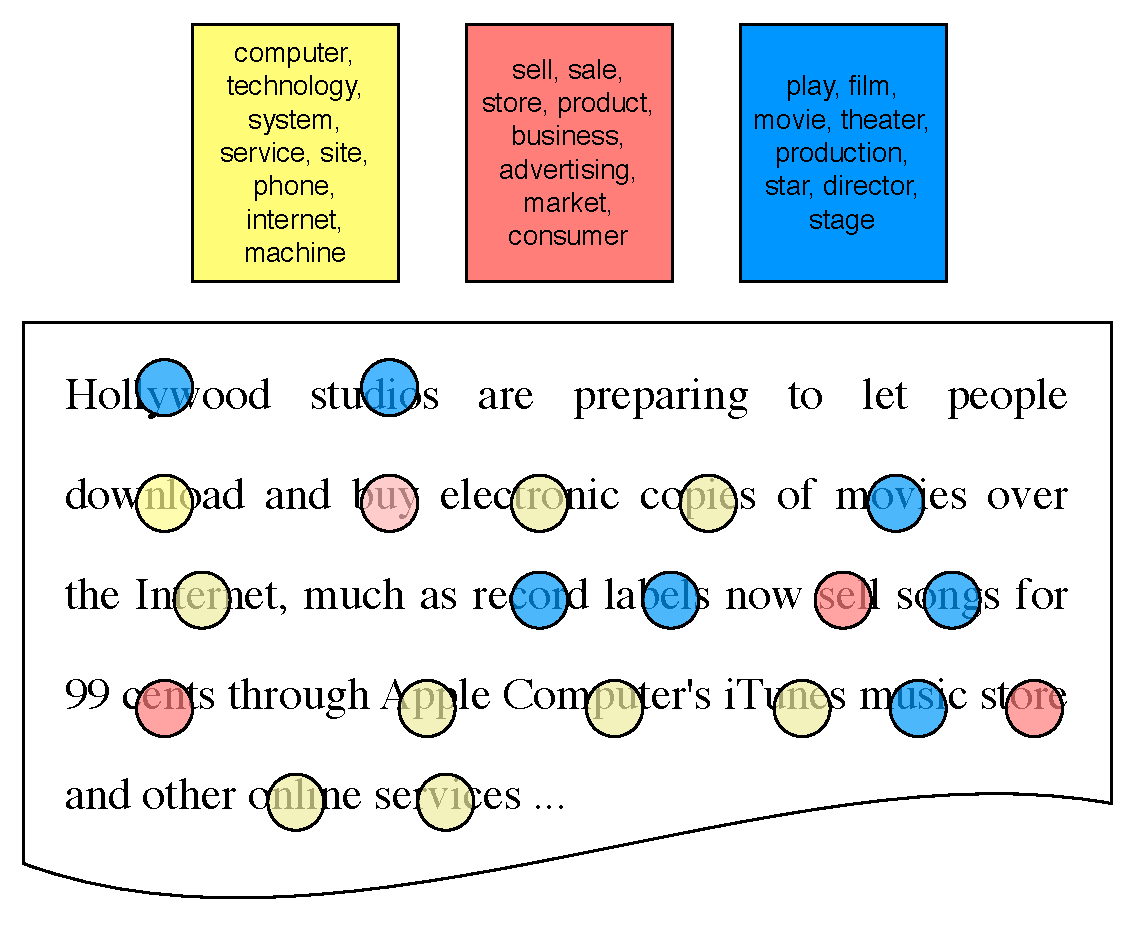
\includegraphics[width=.6\linewidth]{topic_models/inference_3}  }


\end{frame}

\frame
{
  \frametitle{Generative Model Approach}

\begin{center}
\only<1>{ 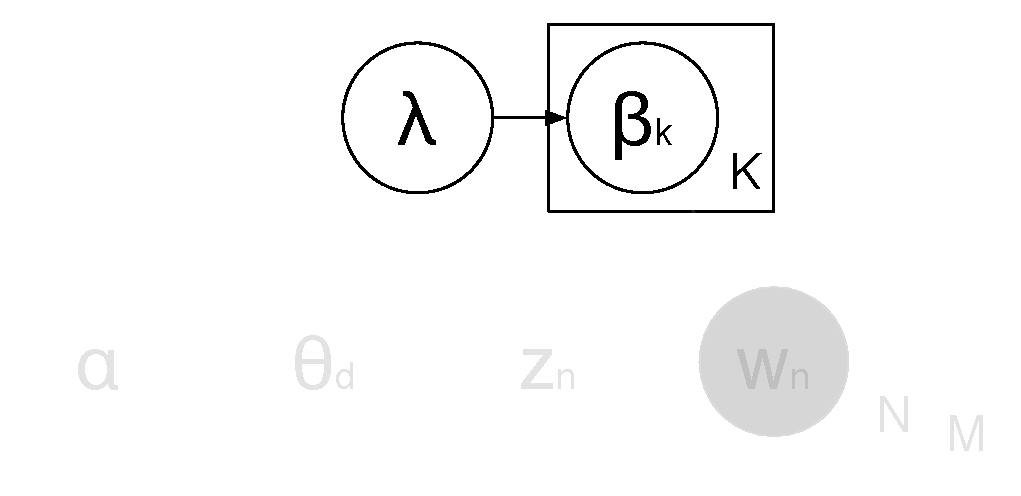
\includegraphics[scale=0.4]{topic_models/lda1.pdf} }
\only<2>{ 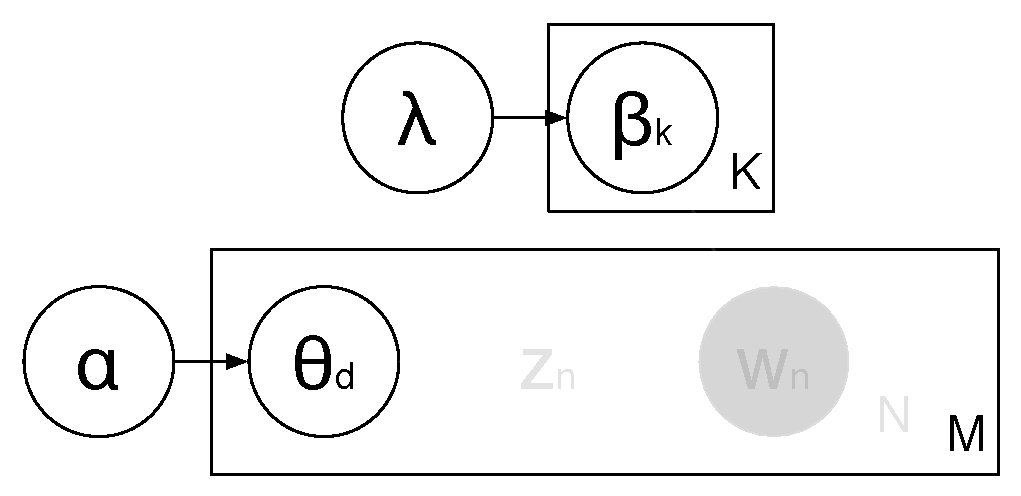
\includegraphics[scale=0.4]{topic_models/lda2.pdf} }
\only<3>{ 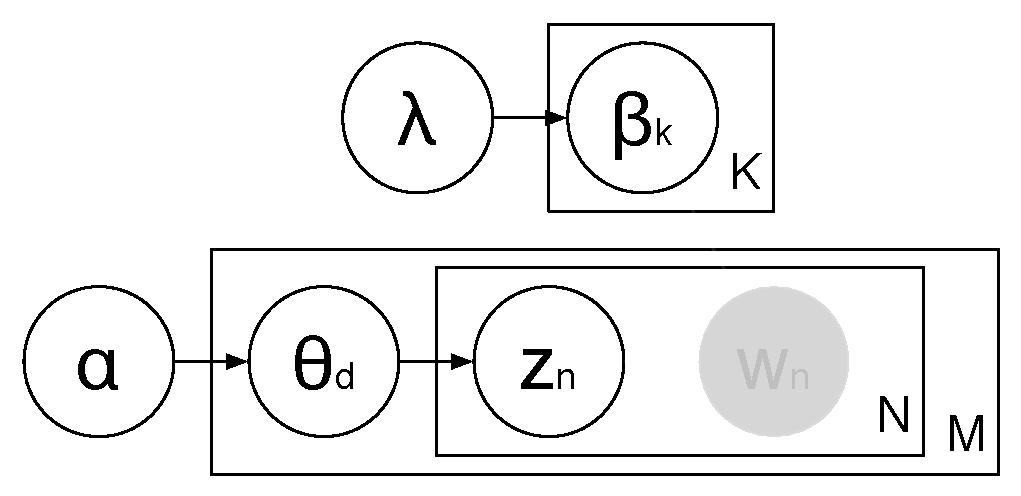
\includegraphics[scale=0.4]{topic_models/lda3.pdf} }
\only<4->{ 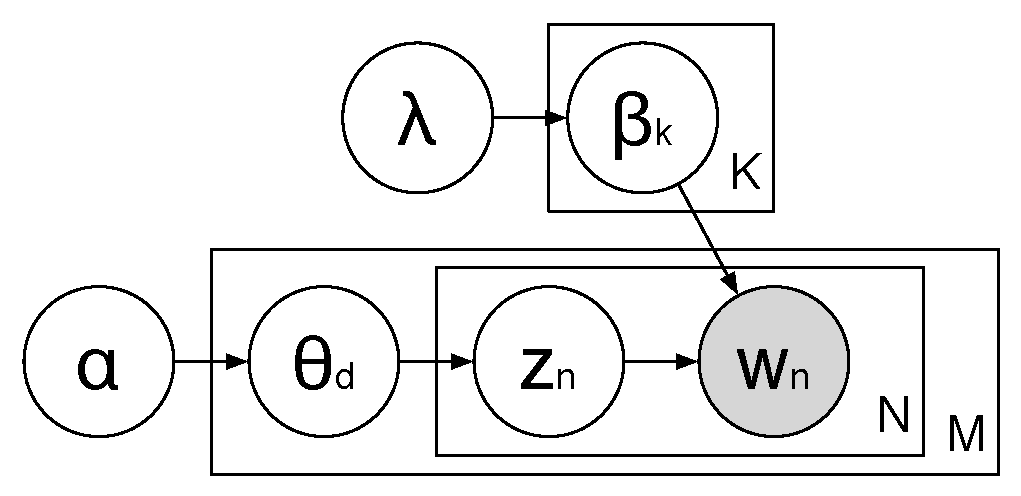
\includegraphics[scale=0.4]{topic_models/lda4.pdf} }
\end{center}

\begin{itemize}
\item<1-> For each topic $k \in \{1, \dots, K\}$, draw a multinomial distribution $\beta_k$ from a Dirichlet distribution with parameter $\lambda$
\item<2-> For each document $d \in \{1, \dots, M\}$, draw a multinomial distribution $\theta_d$ from a Dirichlet distribution with parameter $\alpha$
\item<3-> For each word position $n \in \{1, \dots, N\}$, select a hidden topic $z_n$ from the multinomial distribution parameterized by $\theta$.
\item<4-> Choose the observed word $w_n$ from the distribution $\beta_{z_n}$.
\end{itemize}

\only<5->{We use statistical inference to uncover the most likely unobserved variables given observed data.}
}

\fi

\begin{frame}
\frametitle{Topic Models: What's Important}
\begin{itemize}
\item Topic models \only<2>{(latent variables)}
\begin{itemize}
\ifhighlevel
	\item Topics to word types
	\item Documents to topics
\else
	\item Topics to word types---multinomial distribution
	\item Documents to topics---multinomial distribution
\fi
\end{itemize}
\item Focus in this talk: statistical methods
  \begin{itemize}
    \item Model: story of how your data came to be
    \item Latent variables: missing pieces of your story
    \item Statistical inference: filling in those missing pieces
  \end{itemize}
\item We use latent Dirichlet allocation (LDA)~\cite{blei-03}, a fully Bayesian
  version of pLSI~\cite{hofmann-99}, probabilistic version of
  LSA~\cite{landauer-97}
\end{itemize}

\end{frame}

\ifevaluation


\frame{
\frametitle{Evaluation}
\begin{center}
%\only<1>{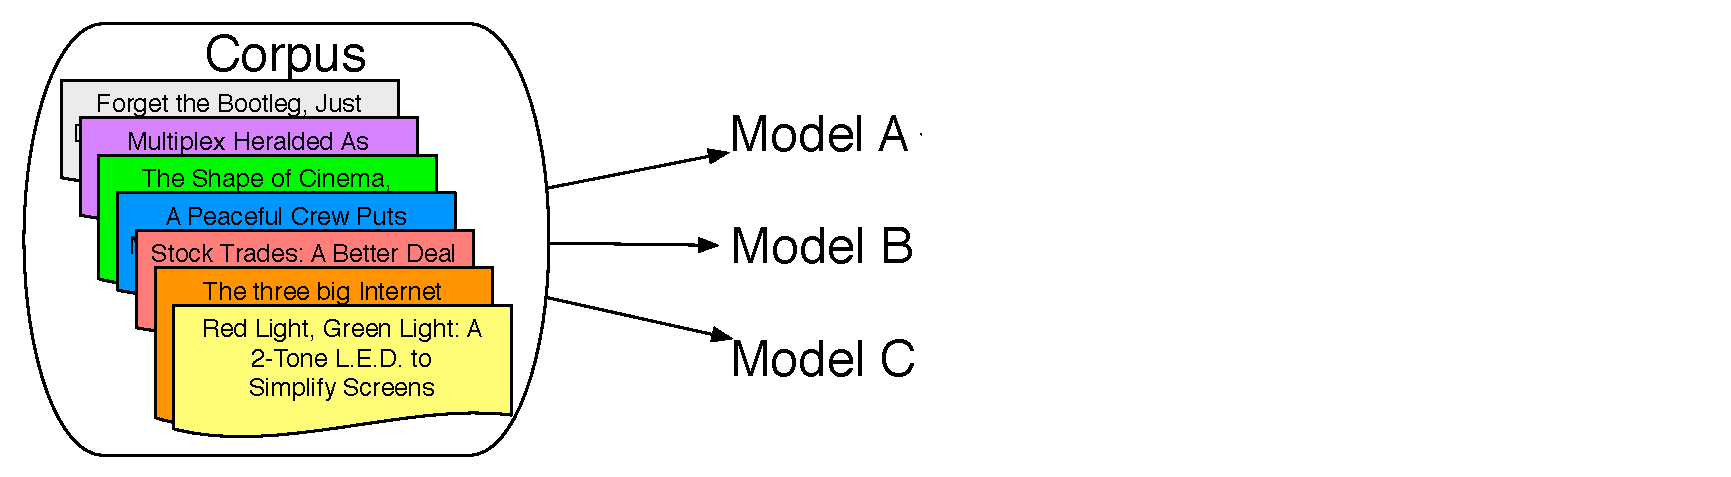
\includegraphics[width=0.9\linewidth]{reading_tea_leaves/figures/heldout_1} }
\only<1>{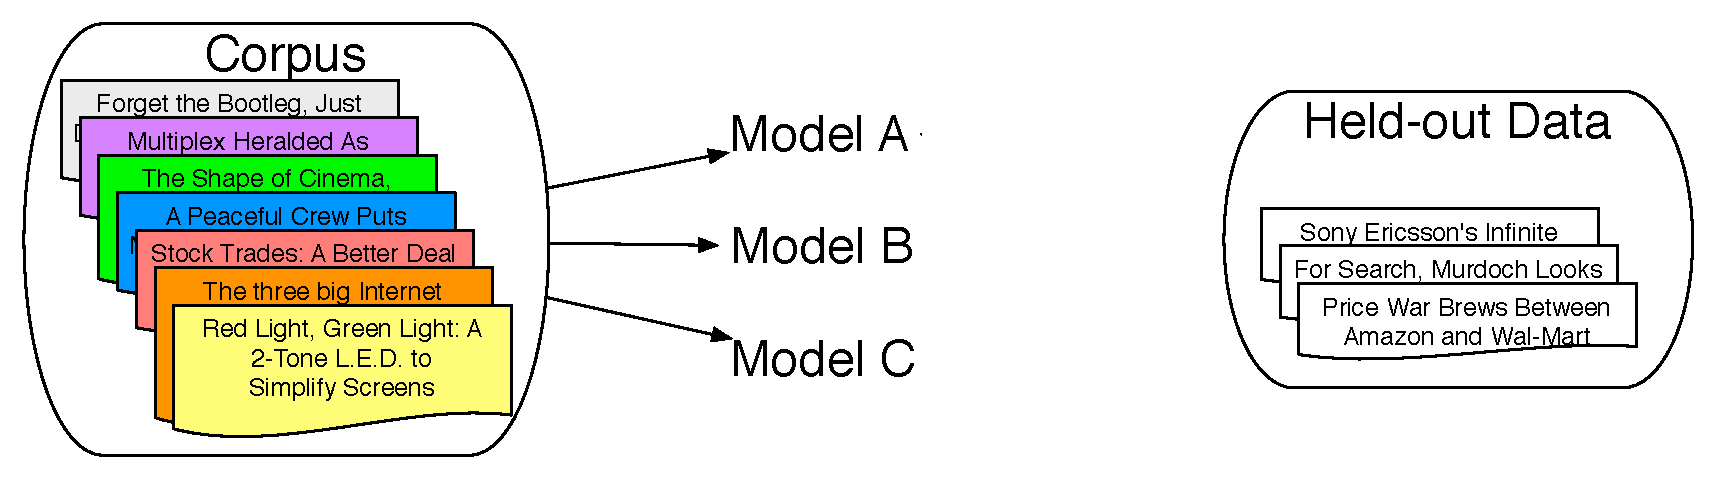
\includegraphics[width=\linewidth]{reading_tea_leaves/figures/heldout_2} }
%\only<3>{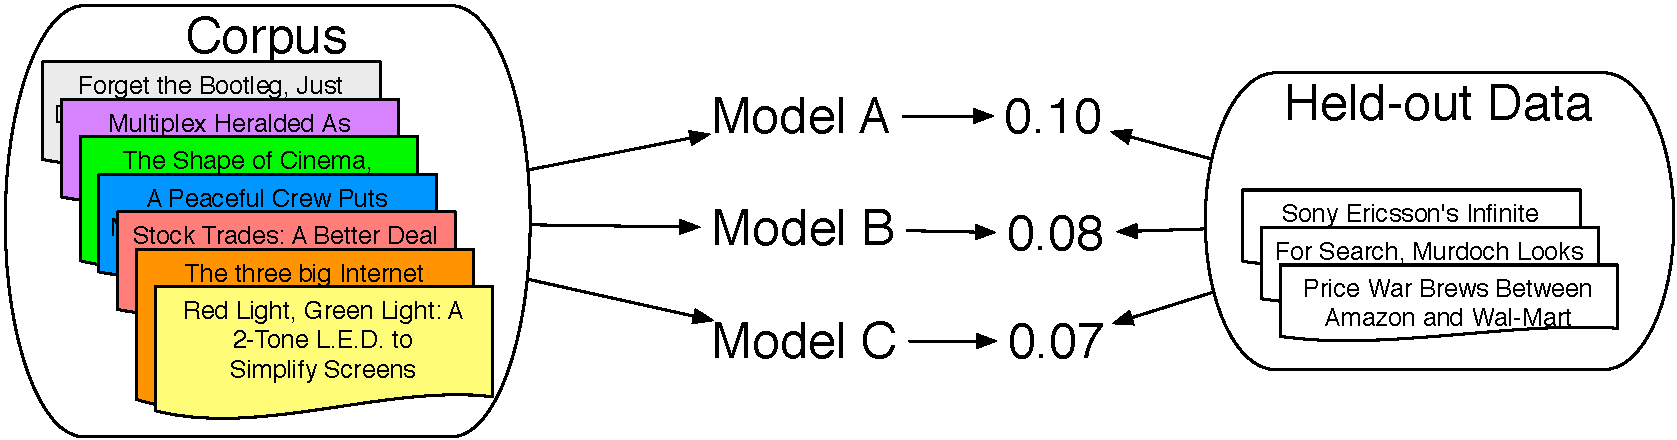
\includegraphics[width=\linewidth]{reading_tea_leaves/figures/heldout_3} }
\only<2>{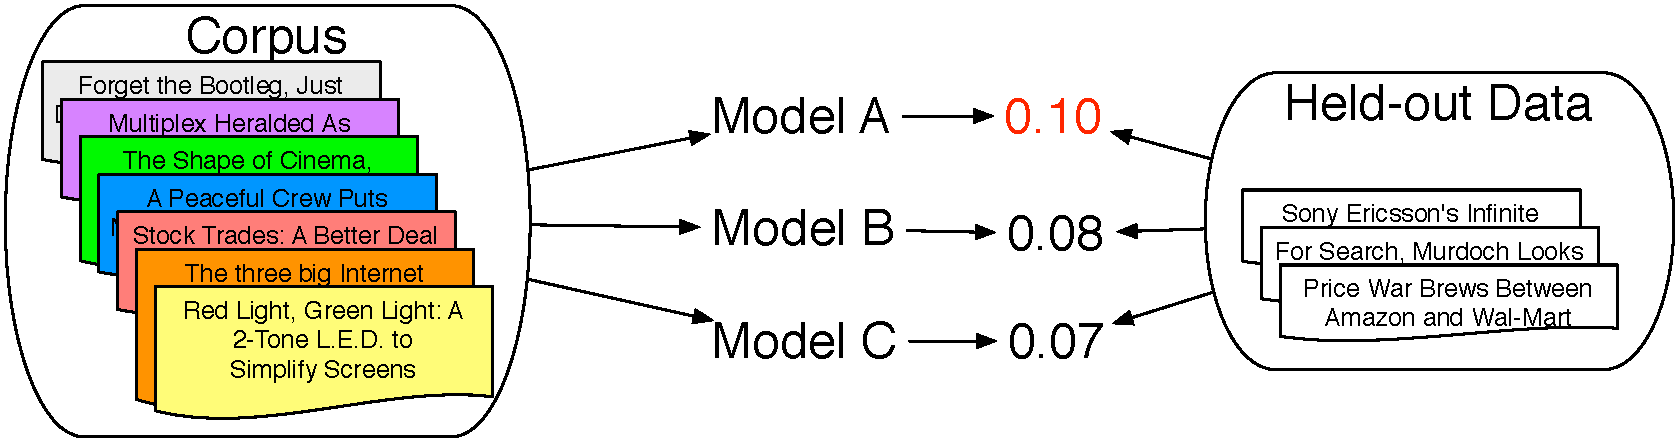
\includegraphics[width=\linewidth]{reading_tea_leaves/figures/heldout_4}  \\
	\large Measures predictive power, not what the topics are}
\end{center}

\begin{center}
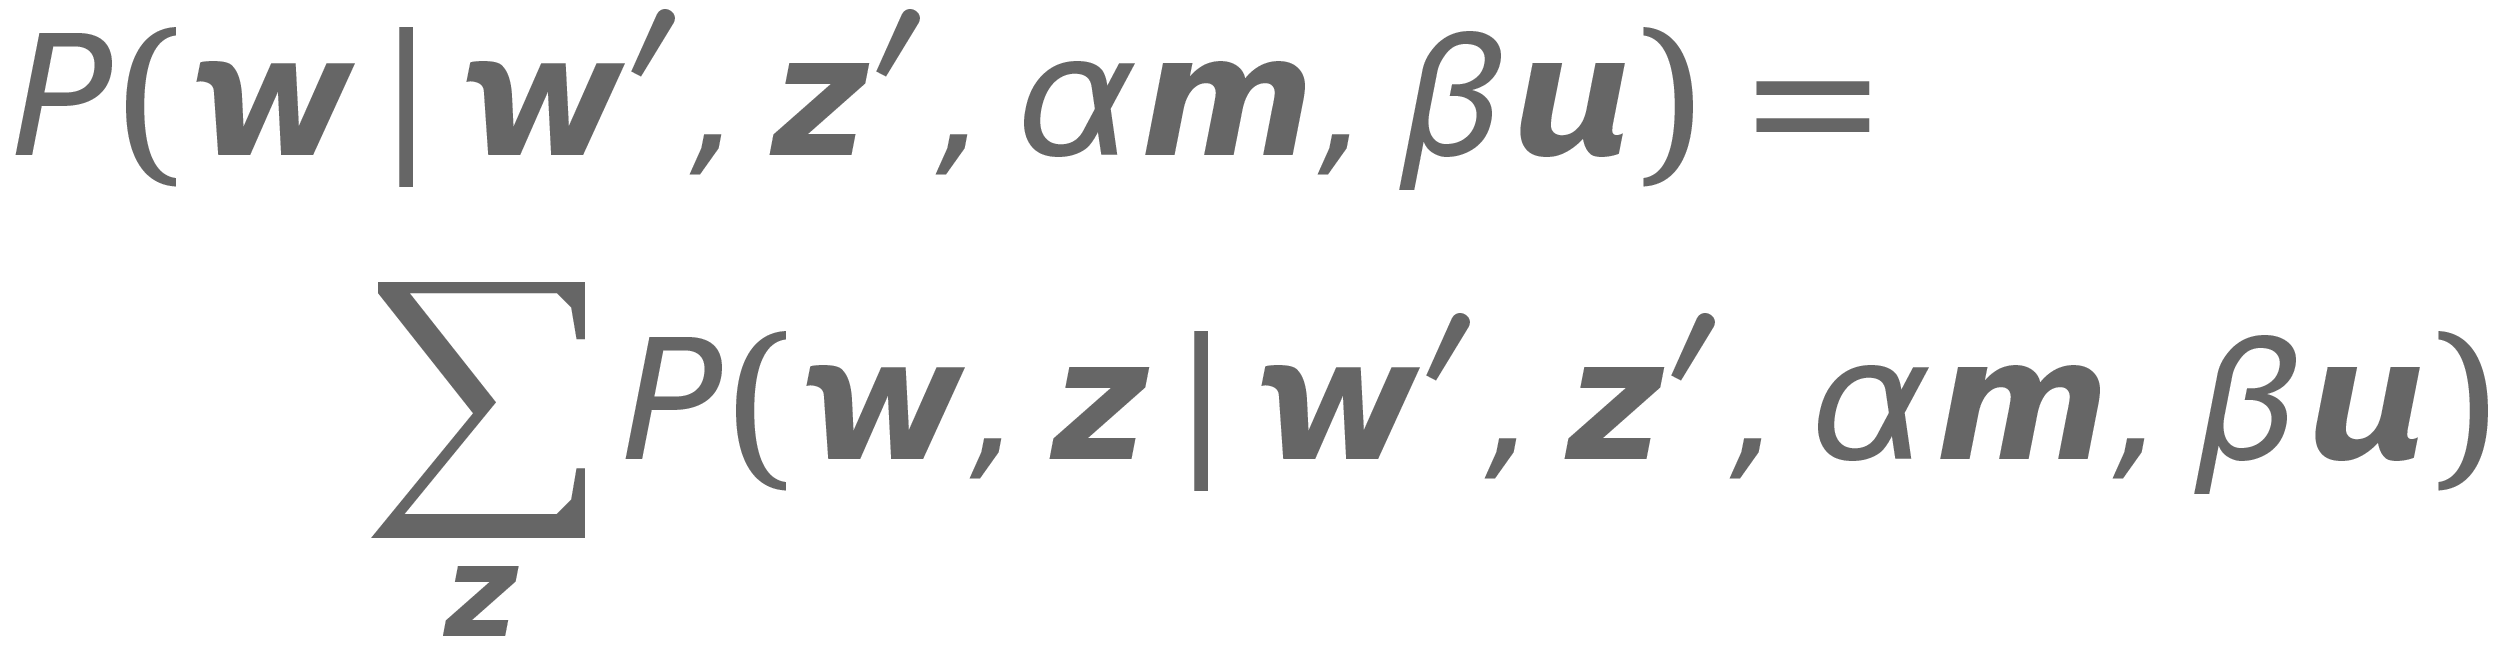
\includegraphics[width=0.5\linewidth]{topic_models/equations/evaluation} \\
How you compute it is important too~\cite{wallach-09b}
\end{center}

}

\frame{
  \frametitle{Word Intrusion}

  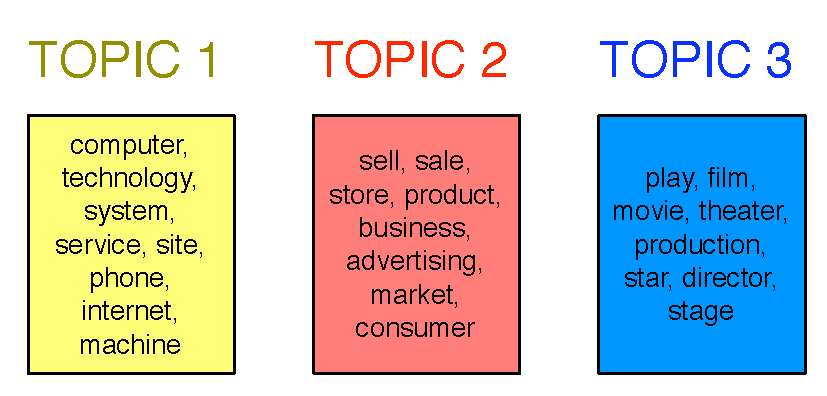
\includegraphics[width=\linewidth]{reading_tea_leaves/figures/nyt_topics_wide}
}


\frame{
  \frametitle{Word Intrusion}

  \begin{enumerate}
    \item Take the highest probability words from a topic

      \begin{block}{Original Topic}
        dog, cat, horse, pig, cow
      \end{block}
\pause
    \item Take a high-probability word from another topic and add it
      \begin{block}{Topic with Intruder}
        dog, cat, \alert<2->{apple}, horse, pig, cow
      \end{block}
\pause
     \item We ask users to find the word that doesn't belong
  \end{enumerate}
\begin{block}{Hypothesis}
If the topics are interpretable, users will consistently choose true intruder
\end{block}
}

\frame{
\frametitle{Word Intrusion}
\begin{center}
\only<1>{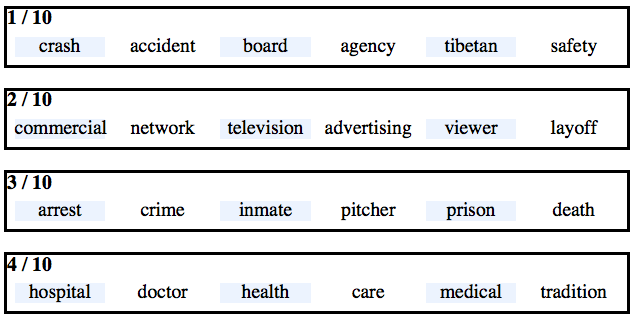
\includegraphics[width=\linewidth]{reading_tea_leaves/tasks/word1}  }
\only<2>{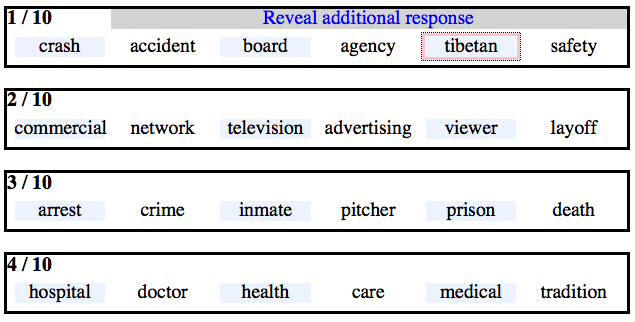
\includegraphics[width=\linewidth]{reading_tea_leaves/tasks/word2}  }
\pause
  \begin{itemize}
    \item Order of words was shuffled
    \item Which intruder was selected varied
    \item Model precision: percentage of users who clicked on intruder
  \end{itemize}

\end{center}
}

\frame{
\frametitle{Word Intrusion: Which Topics are Interpretable?}
  \begin{block}{New York Times, 50 LDA Topics}
    \begin{center}
      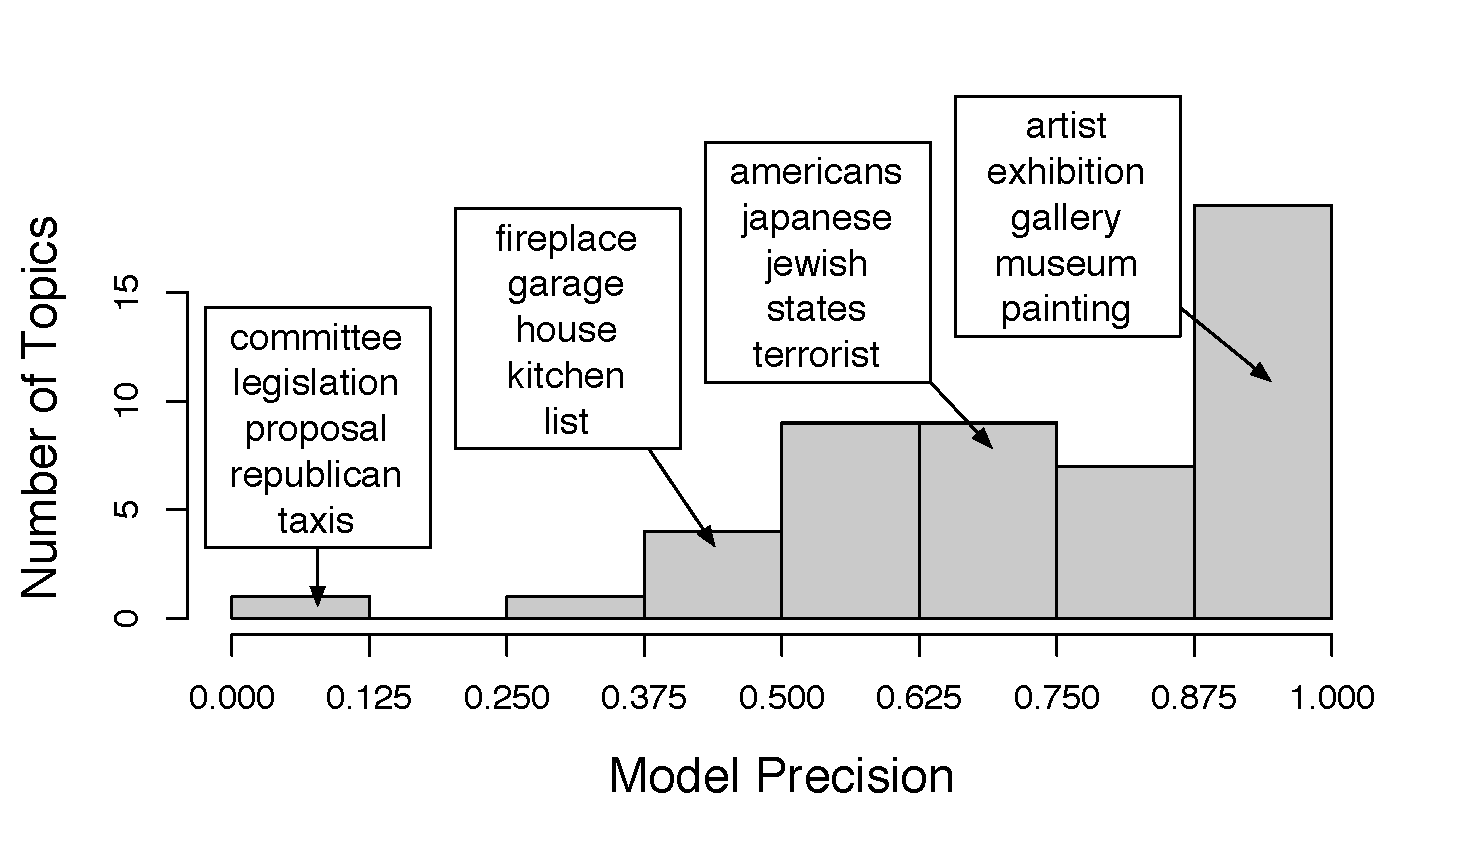
\includegraphics[width=0.8\linewidth]{reading_tea_leaves/figures/topic_precision}
    \end{center}
  \end{block}
  \begin{center}
    Model Precision: percentage of correct intruders found
  \end{center}
}



\frame{

\frametitle{Interpretability and Likelihood}
\begin{center}
\only<1>{Model Precision on New York Times}
\only<2>{Topic Log Odds on Wikipedia}
\end{center}

\begin{columns}
\column{.85\linewidth}
\begin{flushright}
  \only<1>{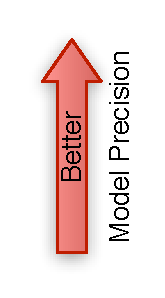
\includegraphics[scale=\graphscale]{reading_tea_leaves/tasks/mp}}
  \only<2>{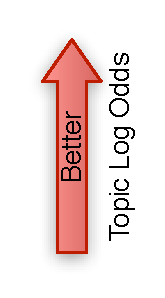
\includegraphics[scale=\graphscale]{reading_tea_leaves/tasks/tlo}}
  \only<1>{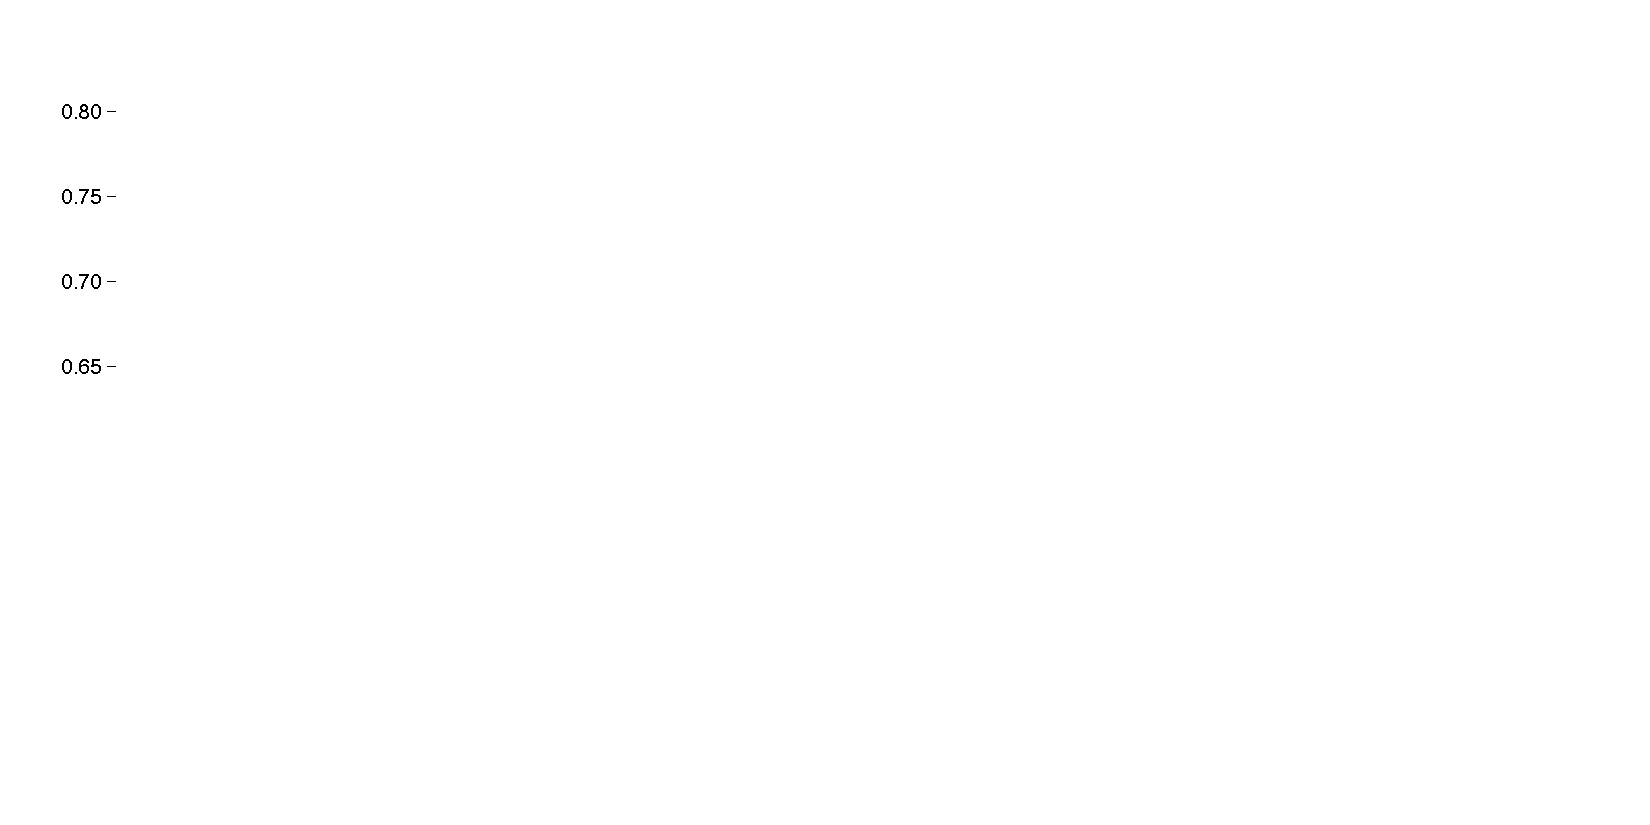
\includegraphics[scale=\graphscale]{reading_tea_leaves/tasks/mp_y}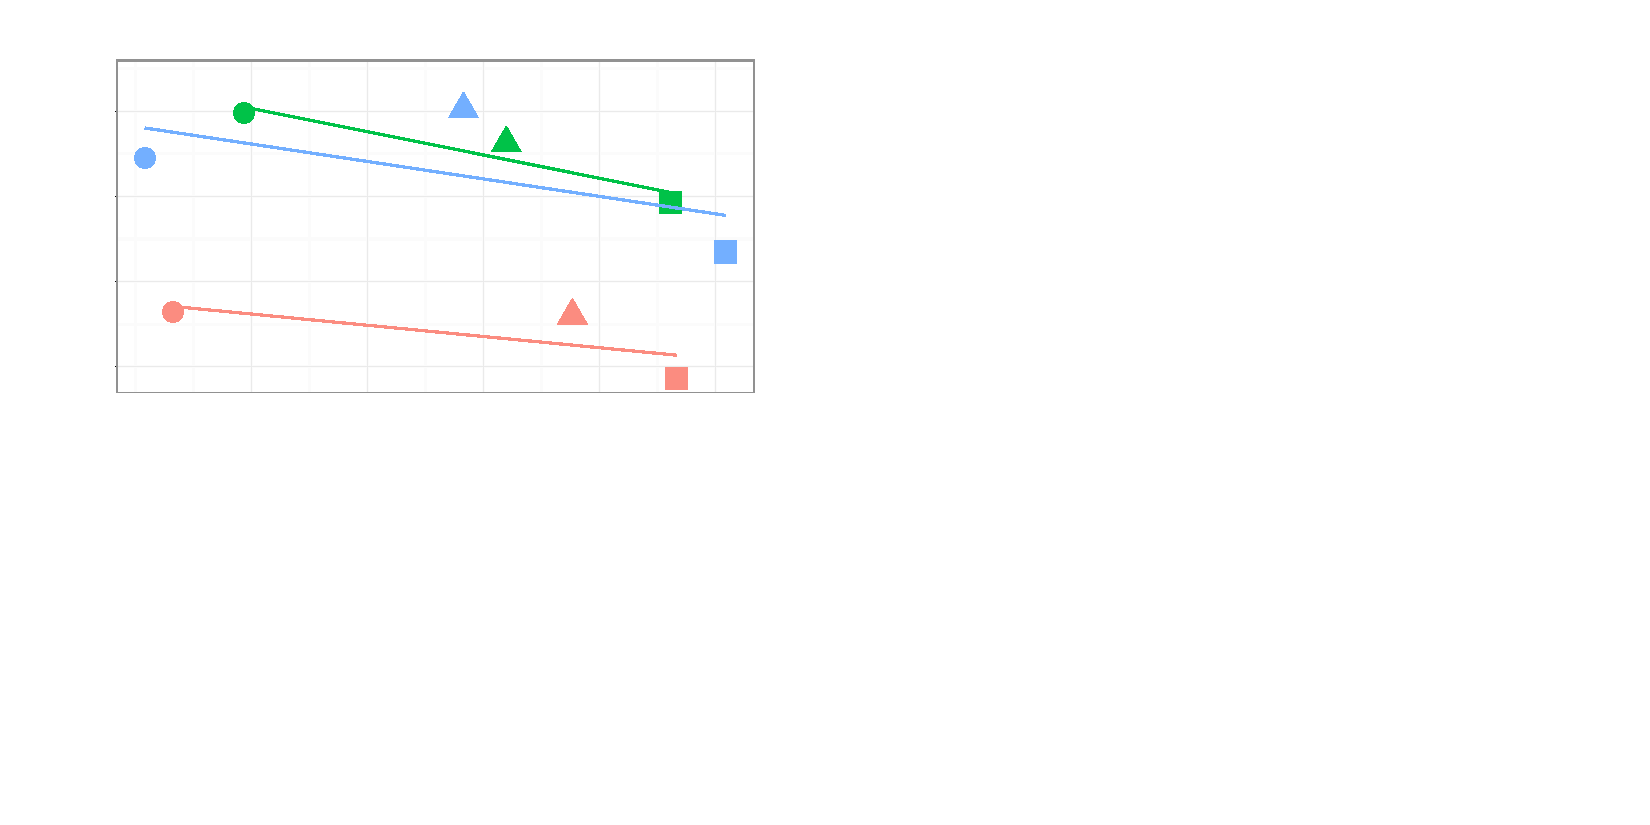
\includegraphics[scale=\graphscale]{reading_tea_leaves/tasks/nyt_mp}}
  \only<2>{
\includegraphics[scale=\graphscale]{reading_tea_leaves/tasks/tlo_y}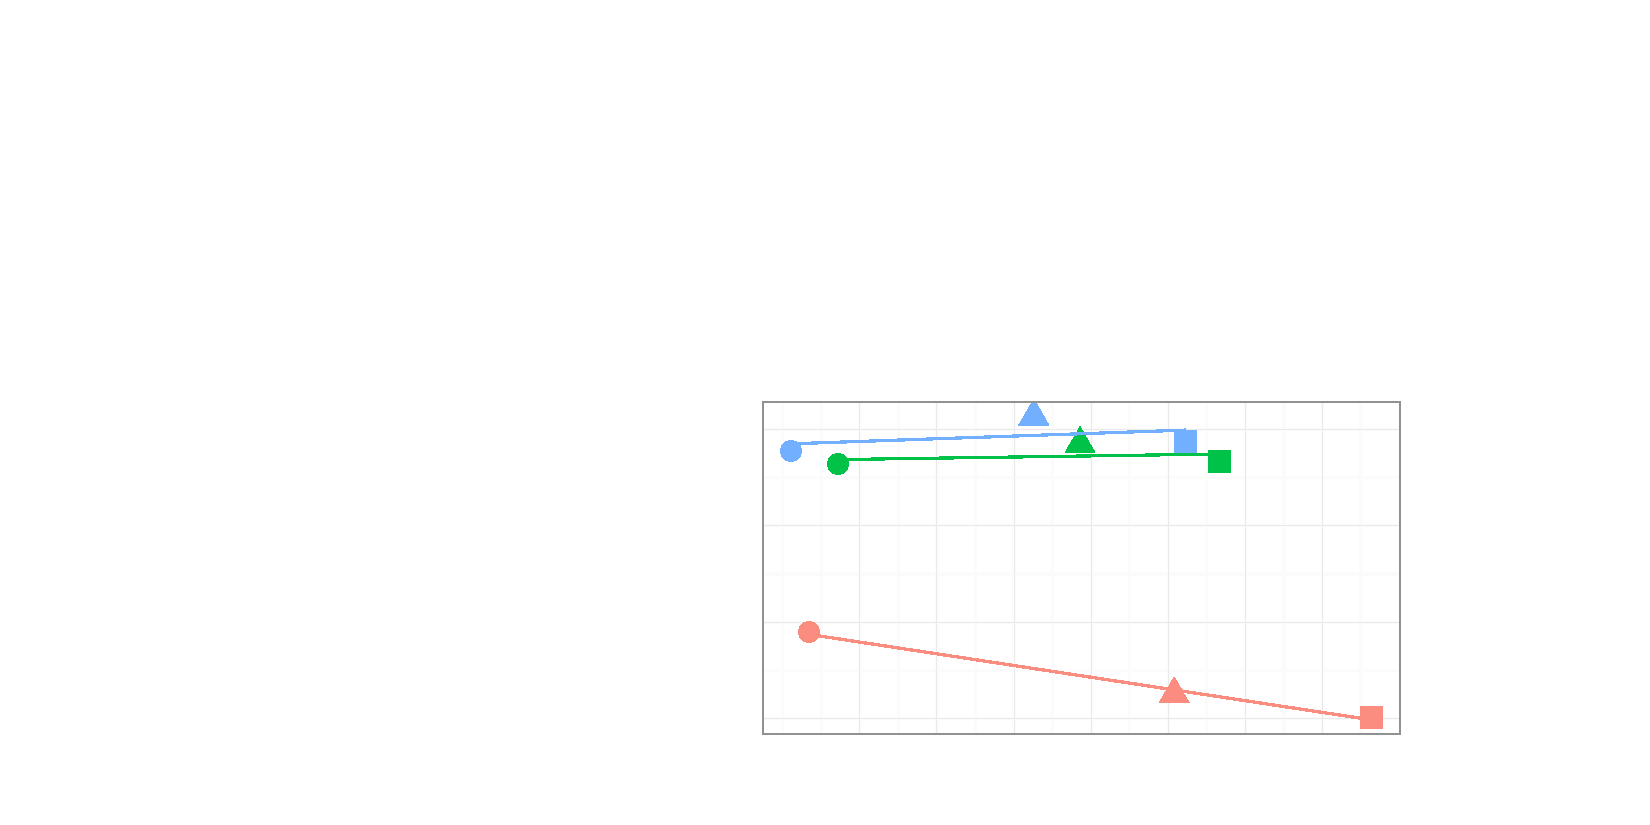
\includegraphics[scale=\graphscale]{reading_tea_leaves/tasks/wiki_tlo}} \\
  \only<1>{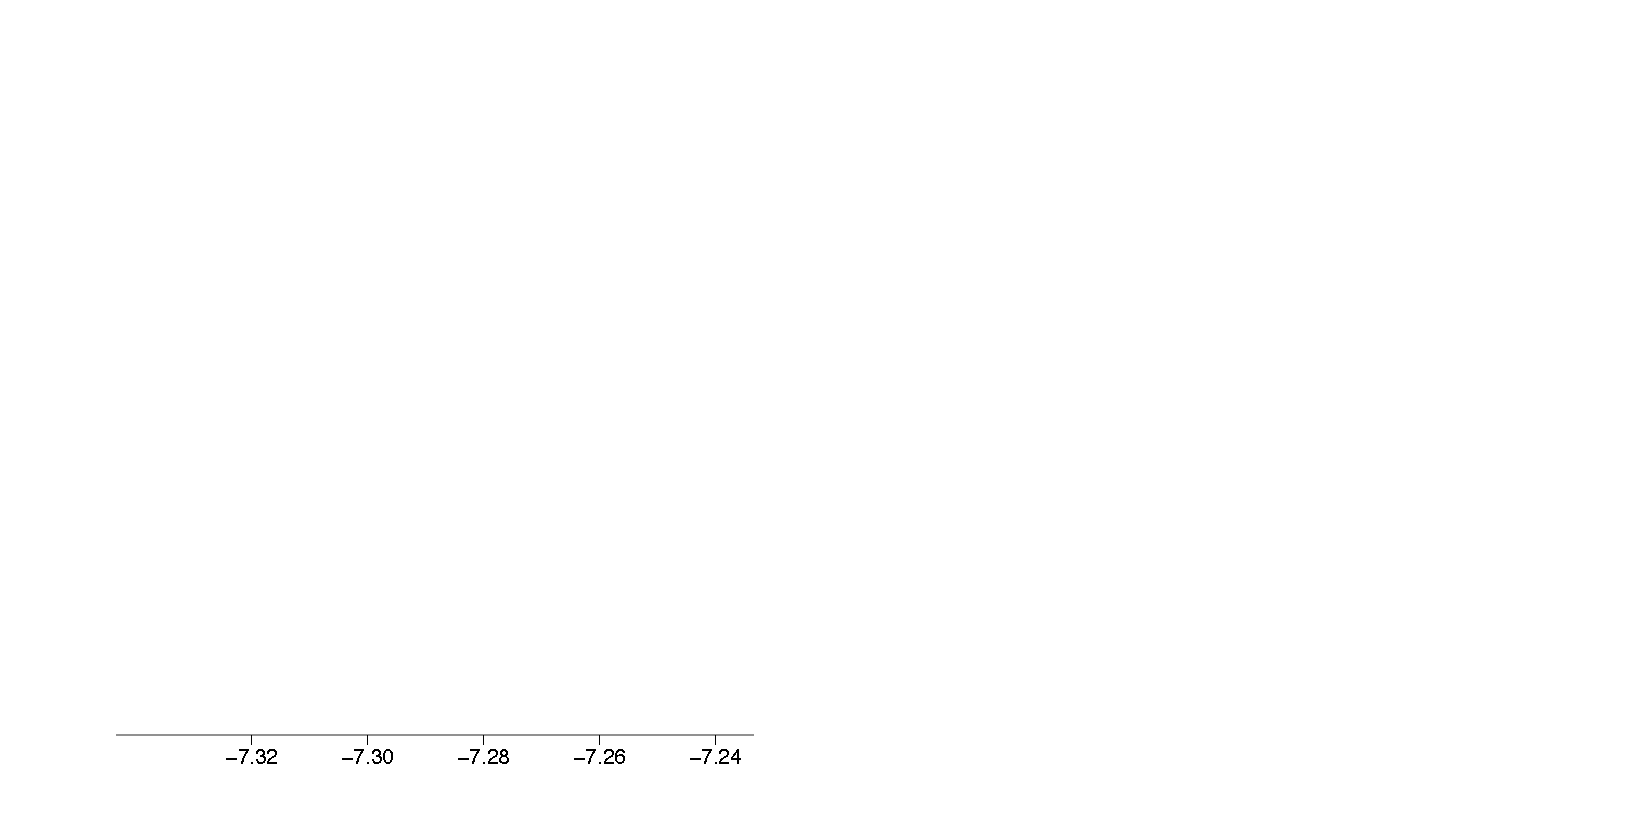
\includegraphics[scale=\graphscale]{reading_tea_leaves/tasks/nyt_x}}
  \only<2>{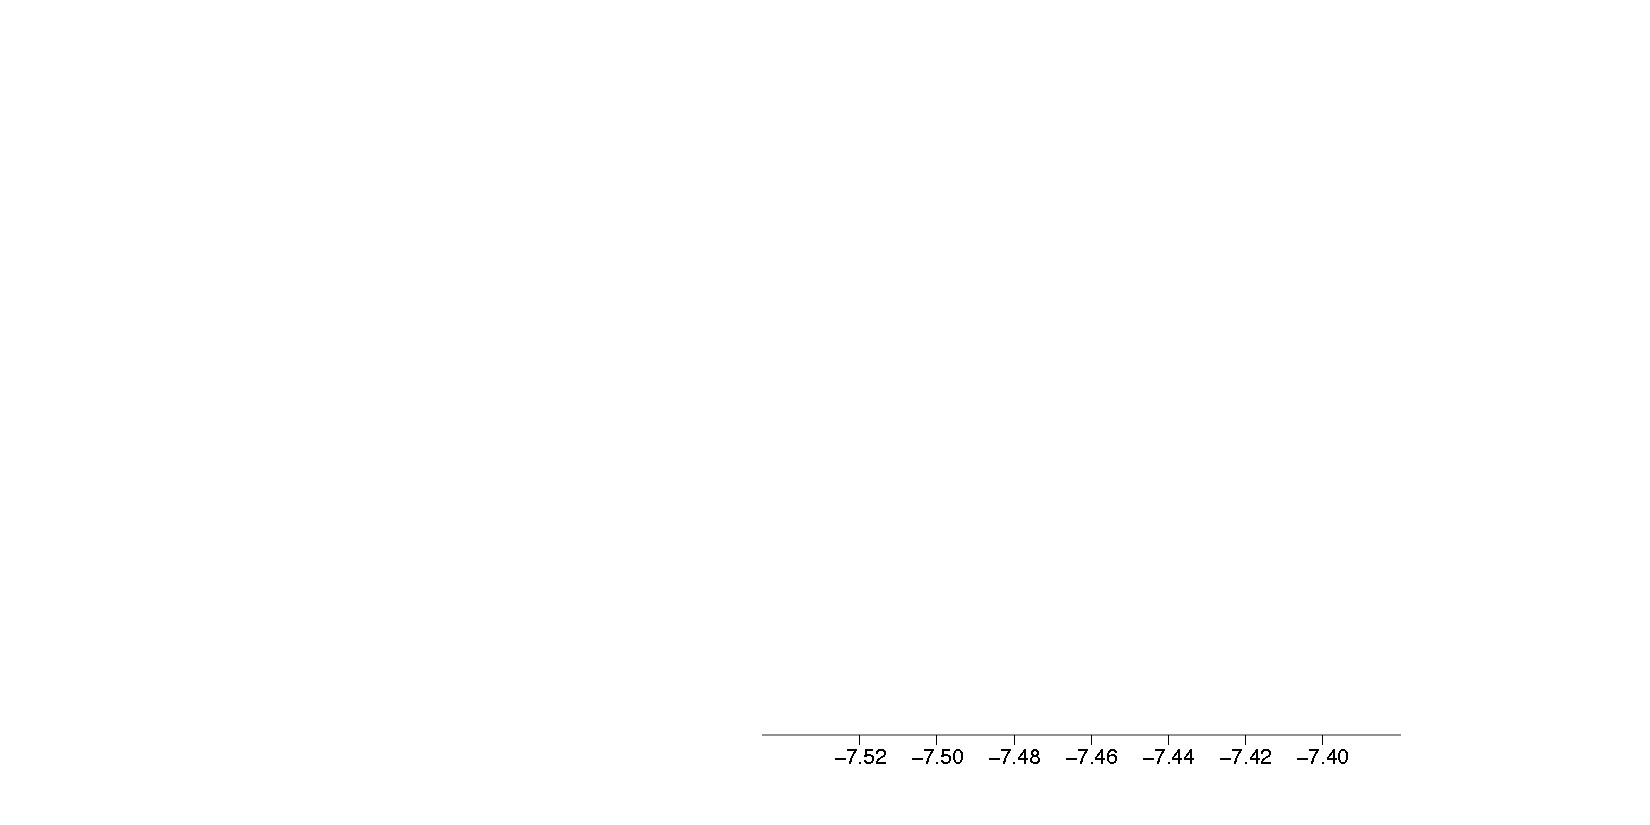
\includegraphics[scale=\graphscale]{reading_tea_leaves/tasks/wiki_x}}
\end{flushright}
\column{.15\linewidth}
  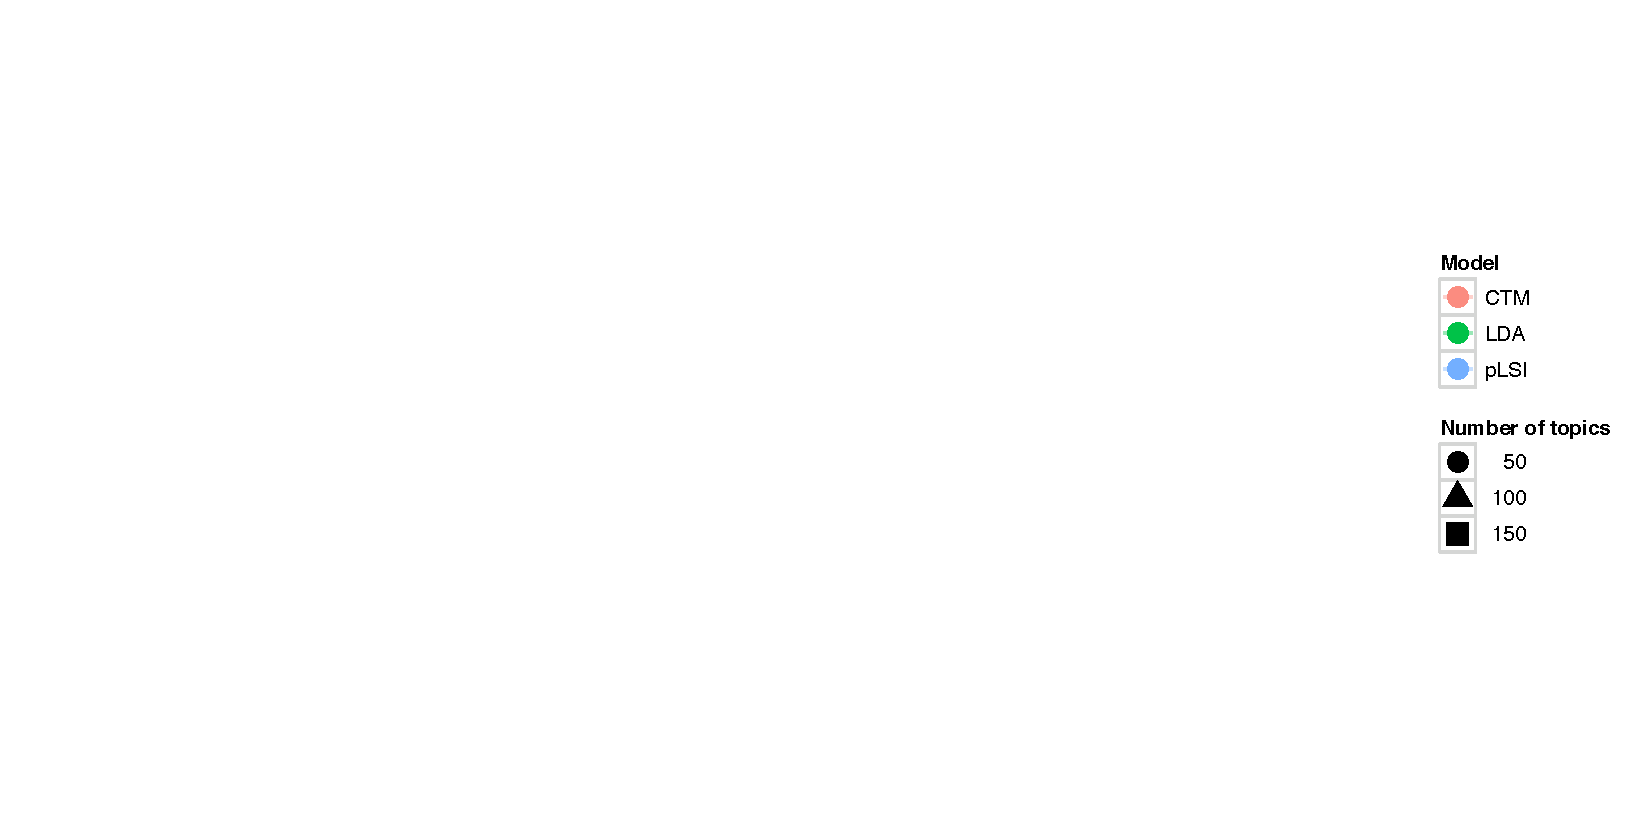
\includegraphics[scale=\graphscale]{reading_tea_leaves/tasks/legend}
\end{columns}
\vspace{-0.75cm}
\begin{center}
  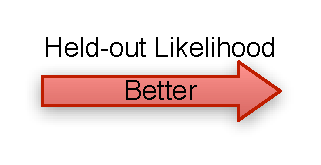
\includegraphics[scale=\graphscale]{reading_tea_leaves/tasks/held-out} \\
\only<1> {within a model, higher likelihood $\not =$ higher interpretability}
\only<2> {across models, higher likelihood $\not =$ higher interpretability}
\end{center}
}


\begin{frame}
  \frametitle{Evaluation Takeaway}

  \begin{itemize}
    \item Measure what you care about~\cite{chang-09c}
      \item If you care about prediction, likelihood is good
\item If you care about a particular task, measure that
    \end{itemize}

\end{frame}

\fi
